\begin{table*}[b]
	\centering
	\renewcommand{\arraystretch}{1.3}
	\begin{tabularx}{\textwidth}{|Y|Y|Y|Y|}
		\hline
		
		\textbf{Scenario 1} & \textbf{Scenario 2} & \textbf{Scenario 3} & \textbf{Scenario 4} \\
		
		\hline
		
		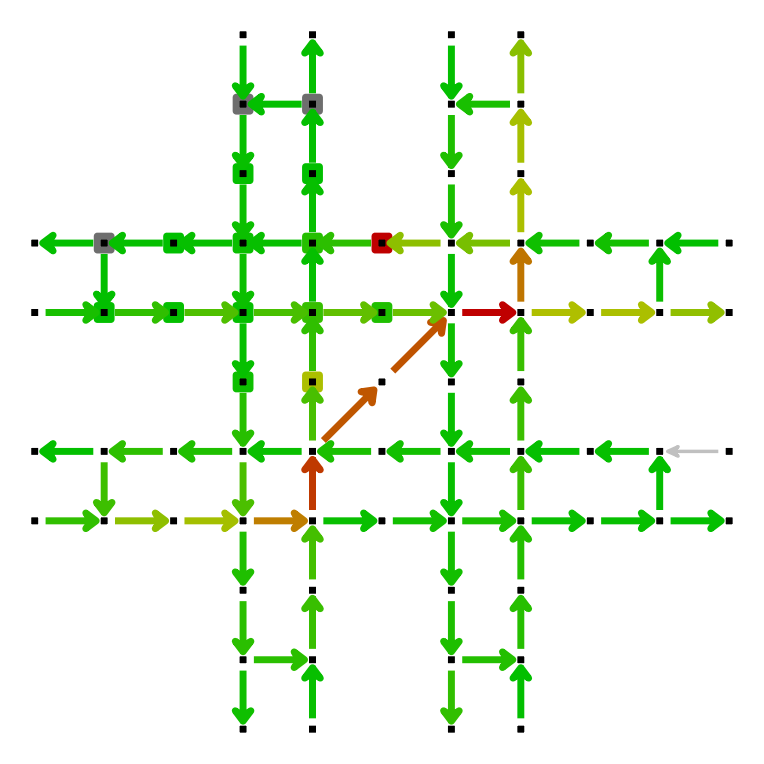
\includegraphics[width=0.23\textwidth, trim=0 0 0 -3]{../gfx/data/E1_003.png} &
		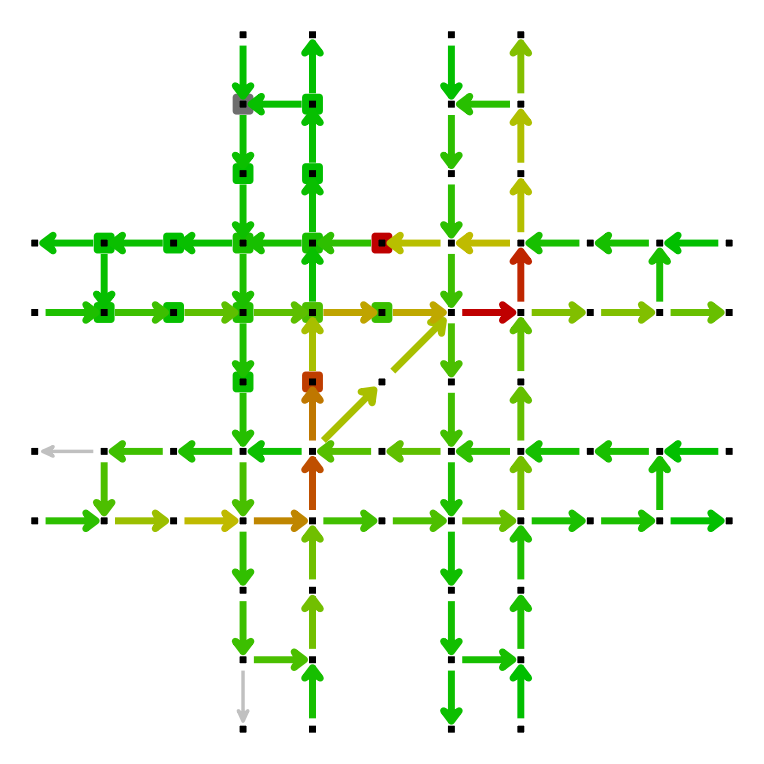
\includegraphics[width=0.23\textwidth, trim=0 0 0 -3]{../gfx/data/E2_003.png} &
		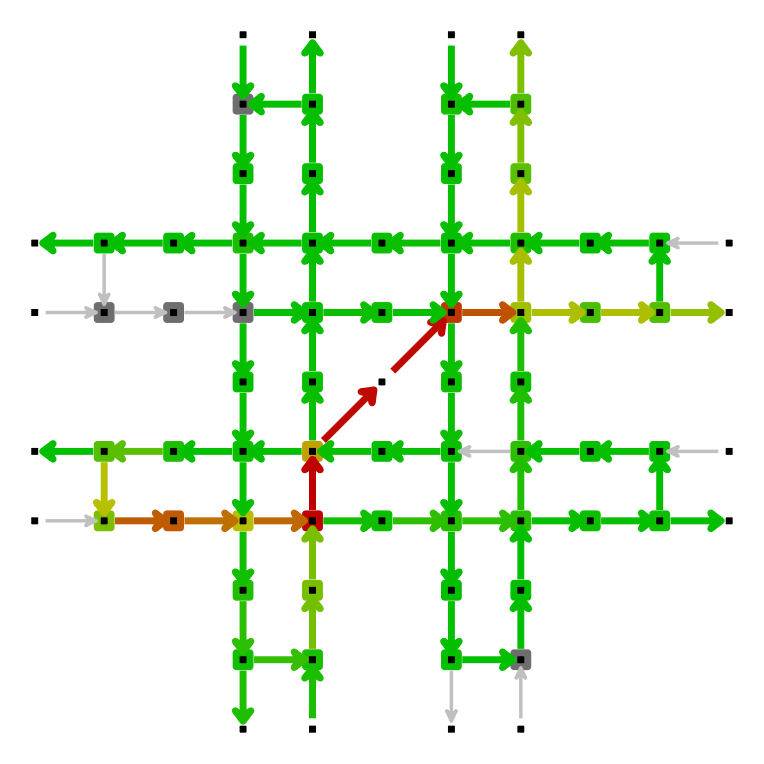
\includegraphics[width=0.23\textwidth, trim=0 0 0 -3]{../gfx/data/E3_003.png} &
		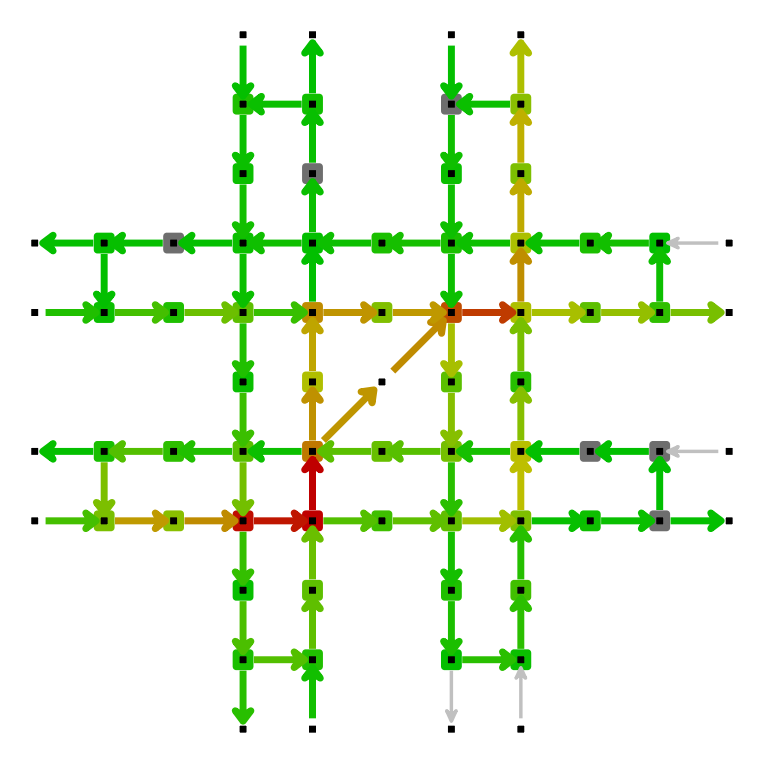
\includegraphics[width=0.23\textwidth, trim=0 0 0 -3]{../gfx/data/E4_003.png} \\
		
		\hline
		
		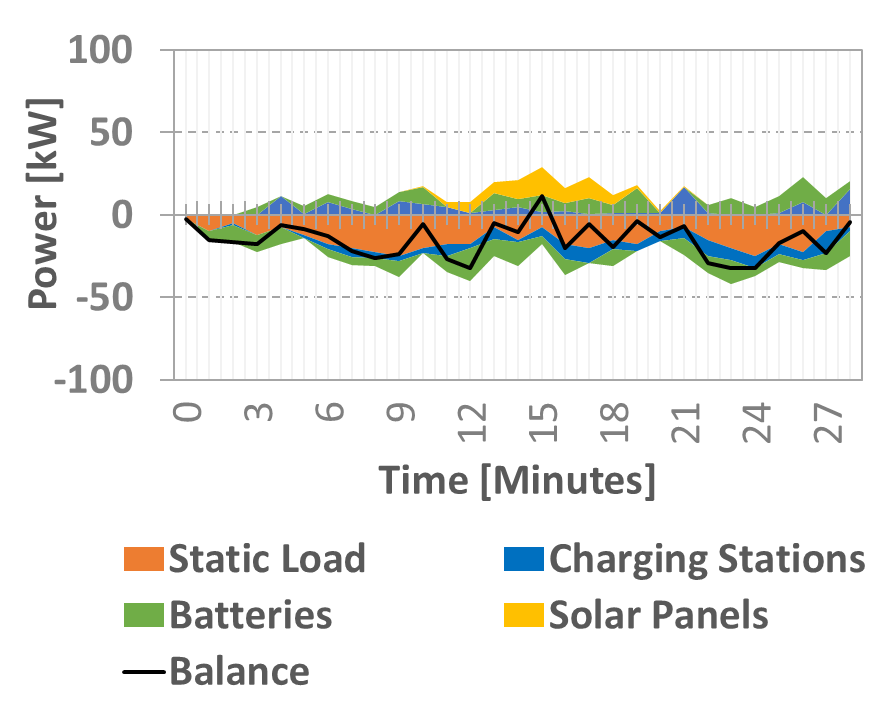
\includegraphics[width=0.23\textwidth, trim=0 0 0 -3]{../gfx/data/E1_001.png} &
		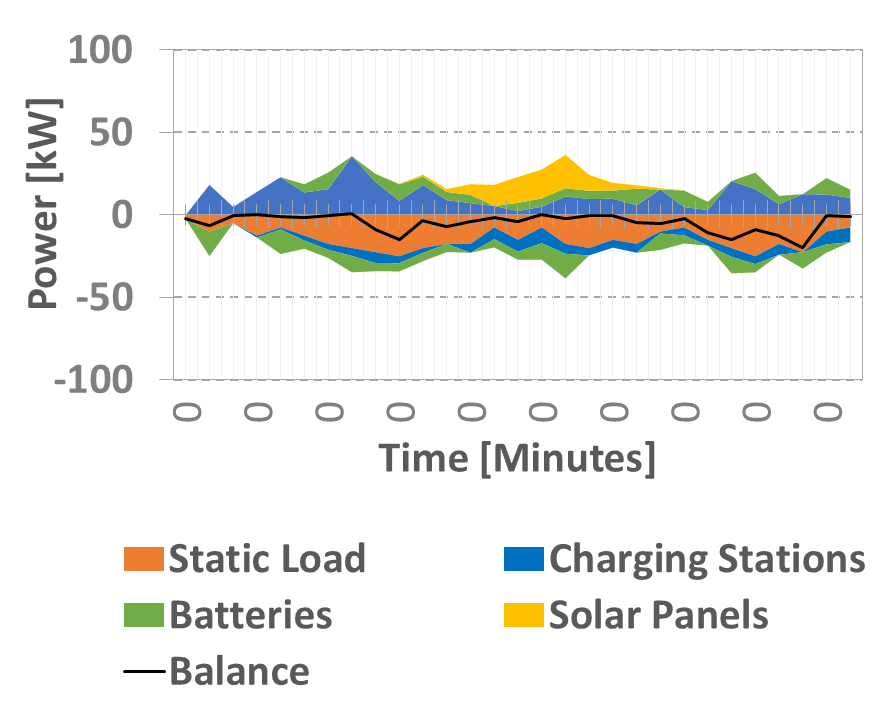
\includegraphics[width=0.23\textwidth, trim=0 0 0 -3]{../gfx/data/E2_001.png} &
		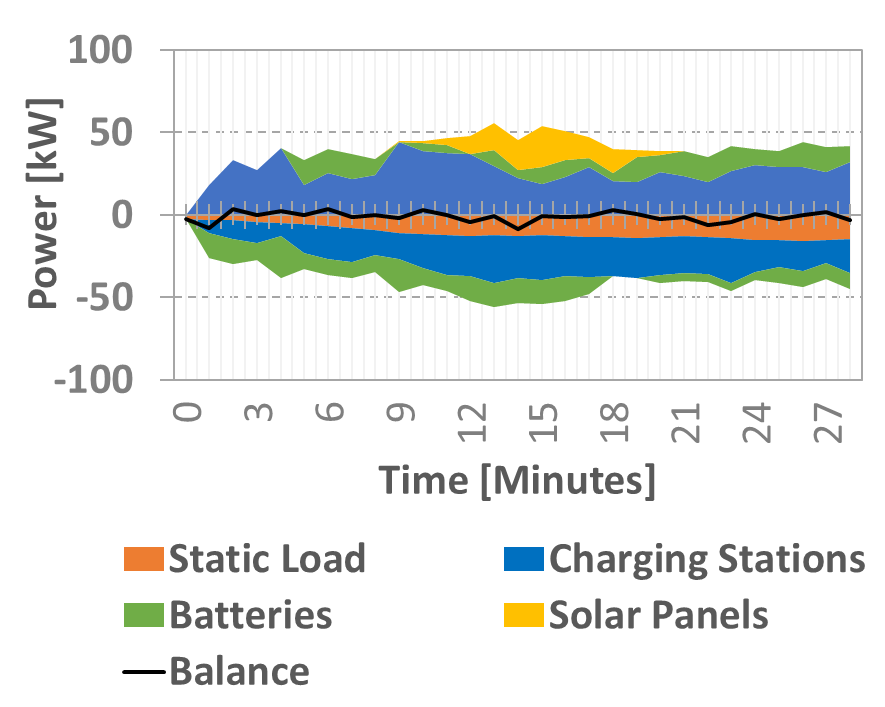
\includegraphics[width=0.23\textwidth, trim=0 0 0 -3]{../gfx/data/E3_001.png} &
		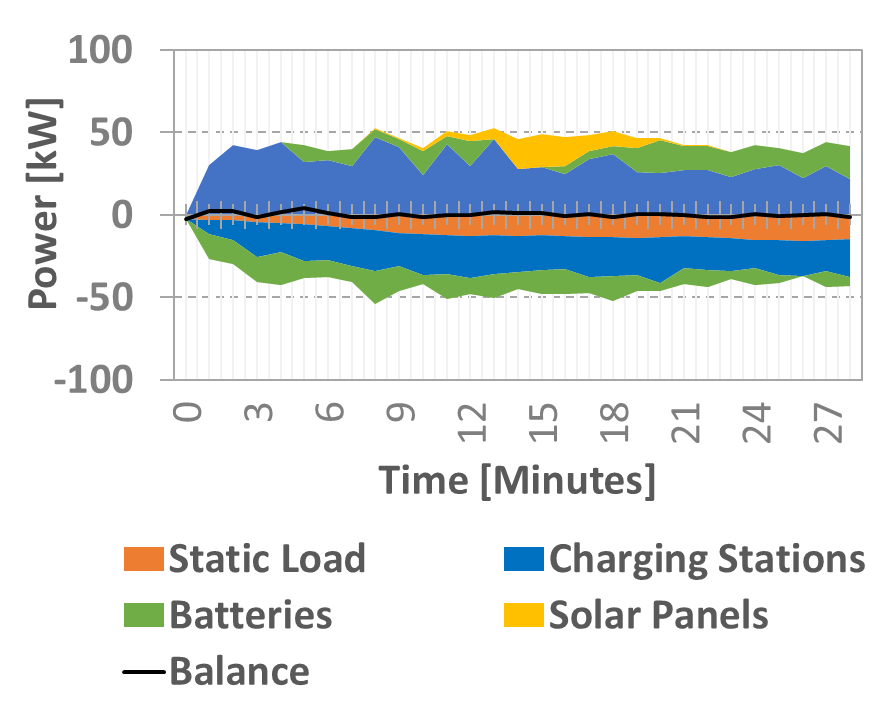
\includegraphics[width=0.23\textwidth, trim=0 0 0 -3]{../gfx/data/E4_001.png} \\
		
		\hline
		
		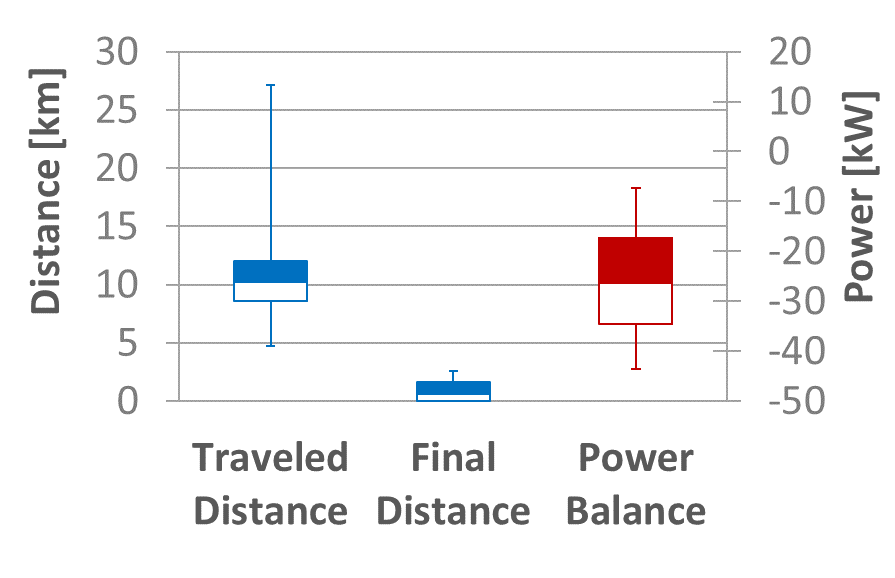
\includegraphics[width=0.23\textwidth, trim=0 0 0 -3]{../gfx/data/E1_002.png} &
		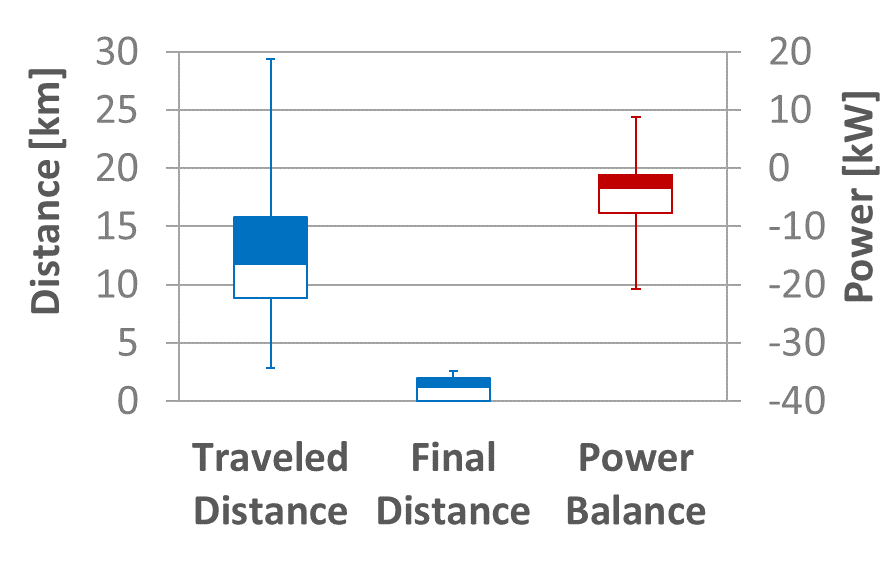
\includegraphics[width=0.23\textwidth, trim=0 0 0 -3]{../gfx/data/E2_002.png} &
		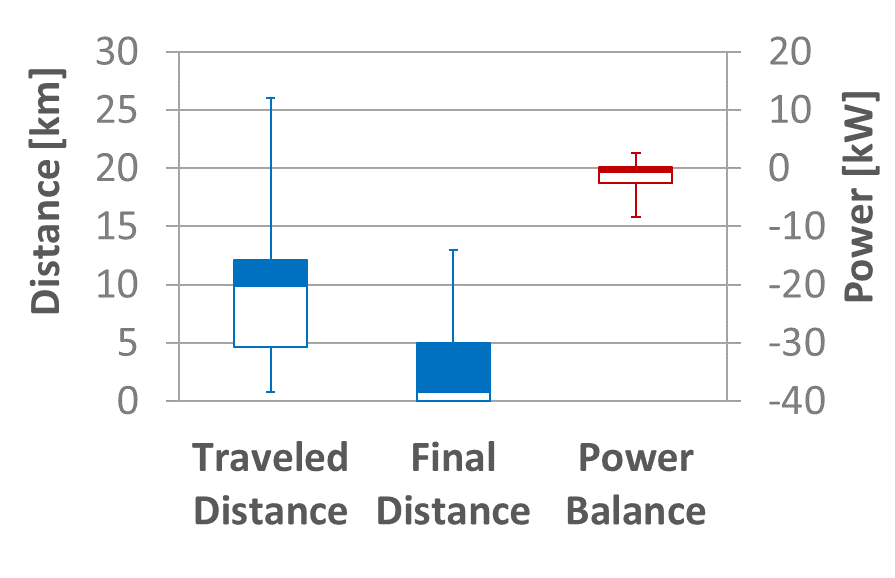
\includegraphics[width=0.23\textwidth, trim=0 0 0 -3]{../gfx/data/E3_002.png} &
		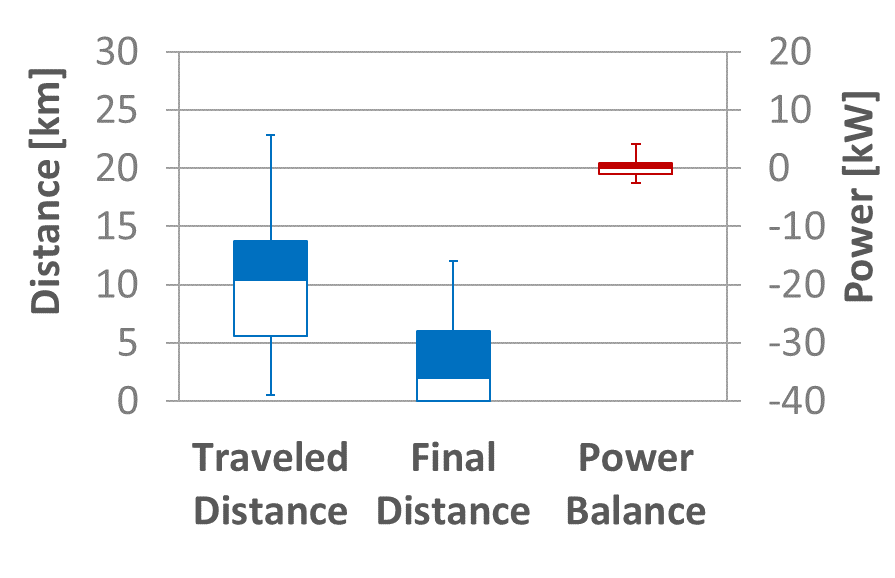
\includegraphics[width=0.23\textwidth, trim=0 0 0 -3]{../gfx/data/E4_002.png} \\
		
		\hline
		
		\begin{tabulary}{4cm}{L|L}
			\textit{Computation time} & 229s \\
			\textit{Memory usage} & 6.03GB \\
		\end{tabulary}
		&
		\begin{tabulary}{4cm}{L|L}
			\textit{Computation time} & 250s \\
			\textit{Memory usage} & 5.27GB \\
		\end{tabulary}
		&
		\begin{tabulary}{4cm}{L|L}
			\textit{Computation time} & 218s \\
			\textit{Memory usage} & 6.41GB \\
		\end{tabulary}
		&
		\begin{tabulary}{4cm}{L|L}
			\textit{Computation time} & 227s \\
			\textit{Memory usage} & 6.75GB \\
		\end{tabulary}
		\\
		
		\hline
	\end{tabularx}
	\caption{Traffic flow graph, power chart, statistics, computation time and memory usage for each scenario.}
	\label{figure:examples}
\end{table*}

\section{Demonstration}
\label{section:evaluation}

To demonstrate the presented approach, we evaluate four example scenario configurations. Generally, all examples are simulated with a time resolution of 60 seconds per simulation step and 30 simulation steps in total, aggregating to a total duration of 30 minutes. The examples evaluate the effects of varying the system objective focus (weight) between the transportation system cost and the power system cost as well as the state of expansion of the power system.

Within the power system $PS$, all scenarios include ten static load components $SL$, five solar panel components $SP$ and five power battery components $PB$ with a specific reference configuration and stage of expansion. 
In all scenarios charging stations as well as four low-voltage nets $LV$ and one medium-voltage net $MV$ with constant reference configurations are employed. 
The stage of expansion of the power system is varied from Scenarios 1-2 to Scenarios 3-4, where solar panel capacities are increased twofold and battery capacities are increased fourfold. Furthermore, in Scenarios 1-2 16 charging stations are employed, in contrast to 56 charging stations in Scenarios 3-4. 

%To model the stage of expansion of the power system, between Scenarios 1-2 and Scenarios 3-4 the configuration of the power system $PS$ is varied in terms of the total number of charging stations as well as solar panel and power battery capacities. Moreover, 

In terms of the transportation system $TS$, the examples feature a total number of 440 cars $C$ and a traffic network $TN$ of 45 kilometers in length and 45 kilometers in width. The cars are distributed equally among three reference configurations, which differ in the cars' initial state of charge (SOC) with 33\%, 66\% and 100\% of the maximum SOC respectively. The origins of cars are drawn randomly from all edges $E$ of the $TN$. Furthermore, the destinations are drawn randomly from a set of the most outward edges of $TN$. Finally, for origins we prefer the lower left sector of $TN$, while for destinations we prefer the upper right.

The results of control optimization are shown in Tab.~\ref{figure:examples}. For each scenario, a traffic flow graph and power chart is provided as well as general statistics and performance characteristics.

\subsubsection*{Scenario 1: Prefer TS, low stage of expansion} 

In terms of traffic flows, results show high frequency of routes utilized representing shortest paths to destinations. Net balance is prone to high fluctuations in load as little equalization of net balances is performed by cars charging/discharging at charging stations.

%In Scenario~1, solar panel and power battery capacities available within the power system are low, while static profiles within the power system have high impact in terms of intermittent power loads. Furthermore, only a low number of charging stations is available. In benefit of achieving the objectives of the transportation system, higher weight is assigned to the costs incurred by the transportation system instead of the power system.

\subsubsection*{Scenario 2: Prefer PS, low stage of expansion}

Results show traffic flows with a higher frequency of edges visited around and on charging stations. Furthermore, compared to Scenario~1, cars utilize shortest path routes to destinations less frequently, which results in marginally higher total distance traveled by cars. Also, net balance is more equalized with cars intermittently discharging at a low number of charging stations.
%In contrast to Scenario~1, in benefit of achieving the objectives of the power system, higher weight is assigned to the costs incurred by the power system instead of the transportation system. 

\subsubsection*{Scenario 3: Prefer TS, high stage of expansion}

%Similar to Scenario~1, when considering traffic flows, 
Traffic flows show a high frequency of routes utilized representing shortest paths to destinations. Overall distance traveled by cars is decreased, while final distance to destination is increased. Compared to Scenario~2, a higher level of equalization of net balance can be observed, due to a higher number of charging stations enabling cars to charge/discharge and higher capacities of solar panels and power batteries.

%In Scenario~3 an incremental stage of expansion of the power system is modeled. For this, higher solar panel and power battery capacities as well as a higher number of charging stations are employed. As electric devices get smarter, the profiles of static loads are more evened out as less intermittent power load peaks occur. In benefit of achieving the objectives of the transportation system, higher weight is assigned to the costs incurred by the transportation system instead of the power system. 

\subsubsection*{Scenario 4: Prefer PS, high stage of expansion}

%Similar to traffic flows observed in Scenario~2, 
Results show cars utilizing shortest path routes less frequently compared to Scenarios~1 and~3, resulting in higher distance traveled and final distance to destination. Compared to Scenario~2 and 3, frequency is distributed more evenly across the traffic network, resulting in higher frequency of edges visited around and on charging stations. Consequently, due to cars charging/discharging at a high number of charging stations, in contrast to Scenario~3, net balances are more equalized.

%In Scenario 4 higher weight is assigned to the costs incurred by the power system instead of the transportation system. 